\section{Présentation des interfaces web clés}
\label{sec:interfaces-web}
Les douze captures suivantes ont été réalisées le 13 septembre 2026 dans un navigateur, à partir des gabarits Blade et de la feuille de style du projet. Un rendu local isolé leur fournit des comptes, offres et candidatures fictifs, sans connexion à la base métier. Les captures montrent donc les interfaces réellement générées par les vues, avec un jeu de présentation ; elles ne constituent ni des enregistrements de production, ni une recette des opérations de sauvegarde. Les scores affichés sont prédéfinis pour illustrer les composants visuels, et non calculés pendant la prise de vue.

Les images ont une résolution de 1\,280 par 720 pixels. Le manifeste livré précise leur fichier et la page correspondante. Les descriptions se concentrent sur le rôle de l'écran et les actions proposées ; les règles d'autorisation restent celles exposées dans les modèles et dans les routes. Les contrôles visuels de cette série concernent un écran d'ordinateur.

\begin{landscape}
\subsection{Connexion}
{\small\setstretch{1.05}
La page de connexion rassemble l'adresse électronique et le mot de passe dans un formulaire court. L'identité SmartRecruit et l'accès à la création de compte guident l'utilisateur avant l'ouverture de son espace. Cette interface correspond à la carte K01.\par}


\begin{figure}[H]\centering
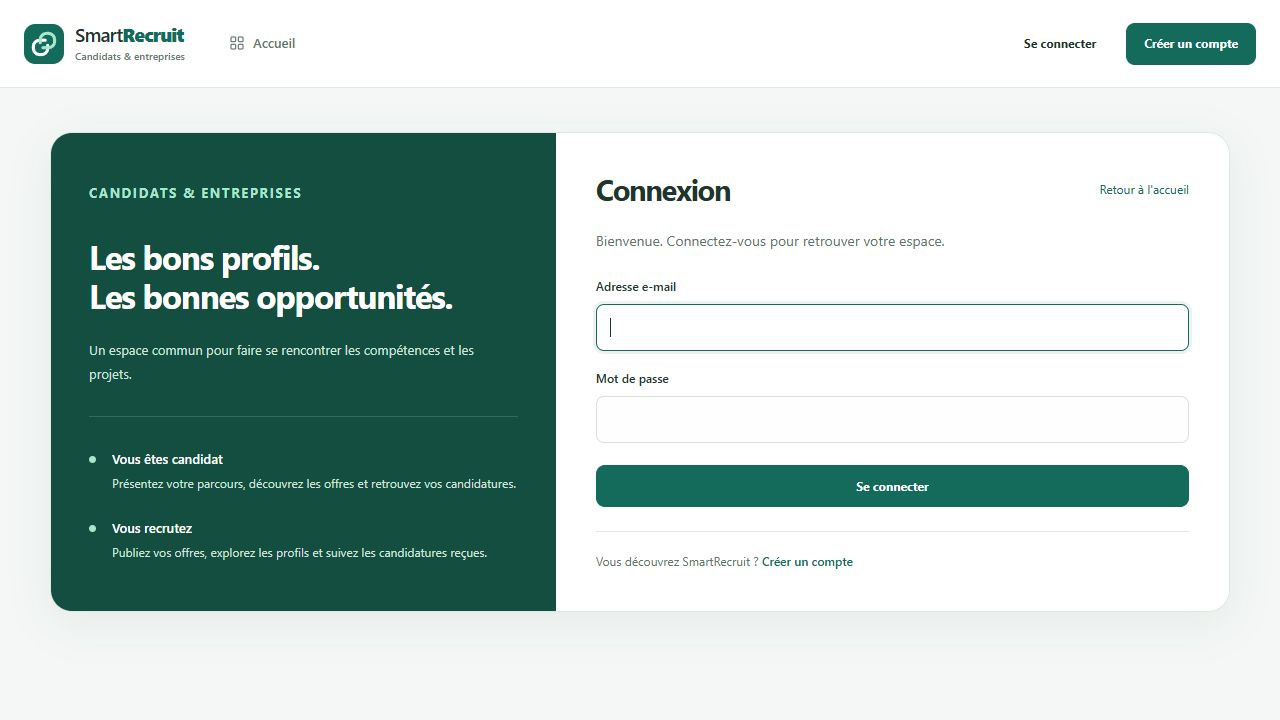
\includegraphics[width=.94\linewidth,height=.74\textwidth,keepaspectratio]{figures/screenshots/01-connexion.png}
\caption{Interface de connexion à SmartRecruit}
\label{fig:interface-01-connexion}\end{figure}
\end{landscape}

\begin{landscape}
\subsection{Choix du profil à l'inscription}
{\small\setstretch{1.05}
L'inscription commence par le choix du type de compte : candidat ou recruteur. Chaque option annonce le parcours associé et prépare le formulaire adapté. Le rôle d'administrateur ne fait pas partie des choix publics.\par}


\begin{figure}[H]\centering
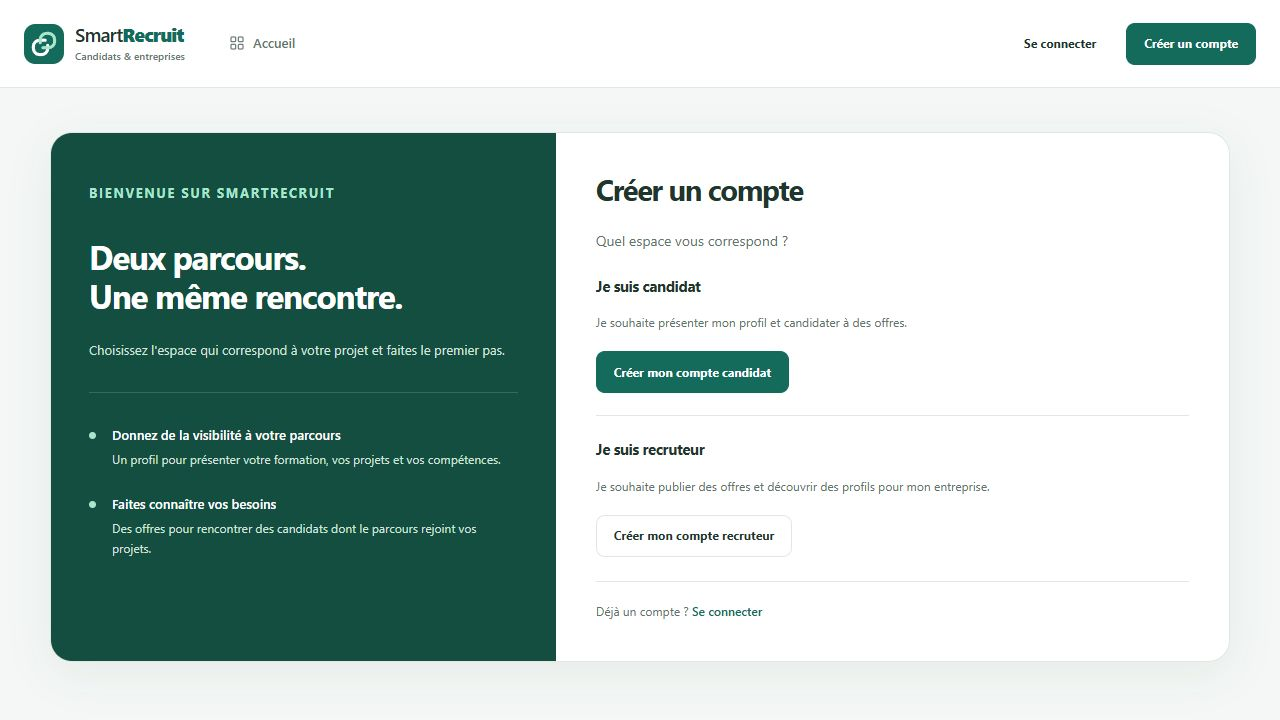
\includegraphics[width=.94\linewidth,height=.74\textwidth,keepaspectratio]{figures/screenshots/02-inscription.png}
\caption{Sélection du type de compte lors de l'inscription}
\label{fig:interface-02-inscription}\end{figure}
\end{landscape}

\begin{landscape}
\subsection{Espace candidat}
{\small\setstretch{1.05}
Le tableau de bord du candidat donne une vue d'ensemble de son profil et de son activité. Les accès aux offres et à la mise à jour du parcours facilitent les actions fréquentes. Le terme candidat employé à l'écran correspond au rôle étudiant du mémoire.\par}


\begin{figure}[H]\centering
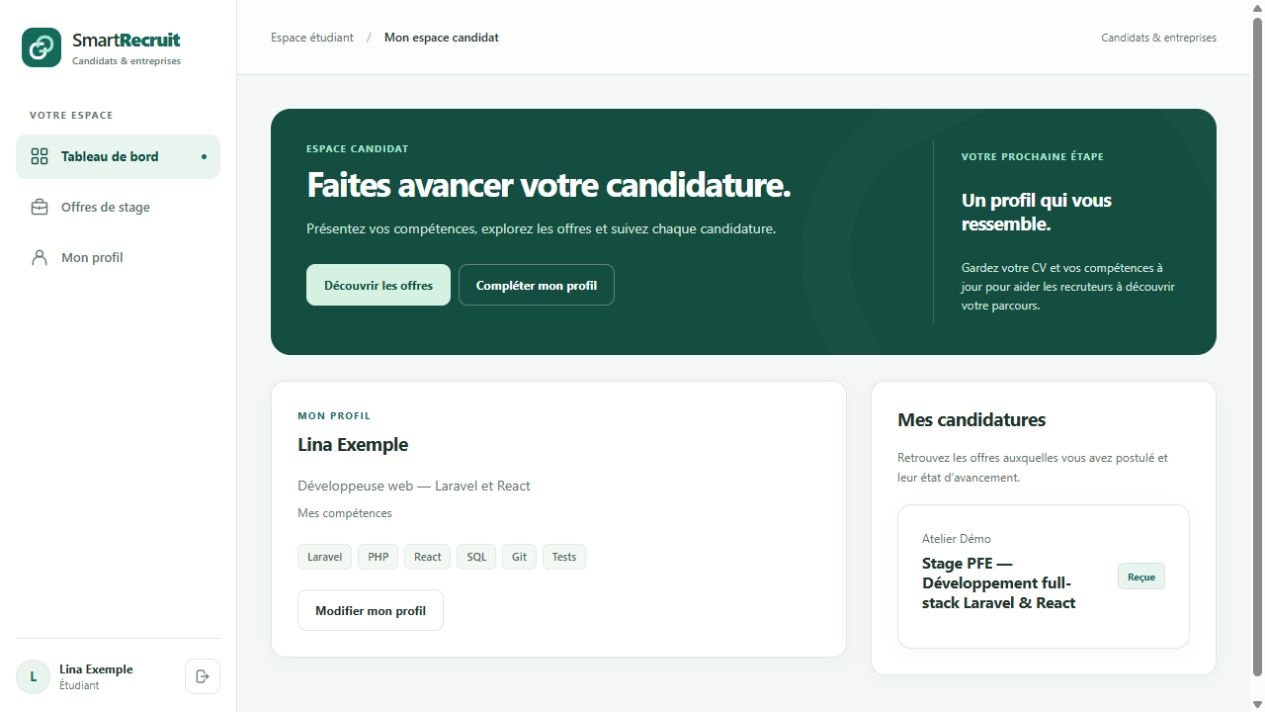
\includegraphics[width=.94\linewidth,height=.74\textwidth,keepaspectratio]{figures/screenshots/05-espace-etudiant.png}
\caption{Tableau de bord du candidat avec données de démonstration}
\label{fig:interface-05-espace-etudiant}\end{figure}
\end{landscape}

\begin{landscape}
\subsection{Profil et informations du CV}
{\small\setstretch{1.05}
La fiche rassemble les informations du parcours, les compétences et les éléments associés au CV. Cette restitution aide à relire les données utilisées lors du rapprochement avec une offre. La possibilité de corriger le profil complète l'extraction automatique décrite par la carte K04.\par}


\begin{figure}[H]\centering
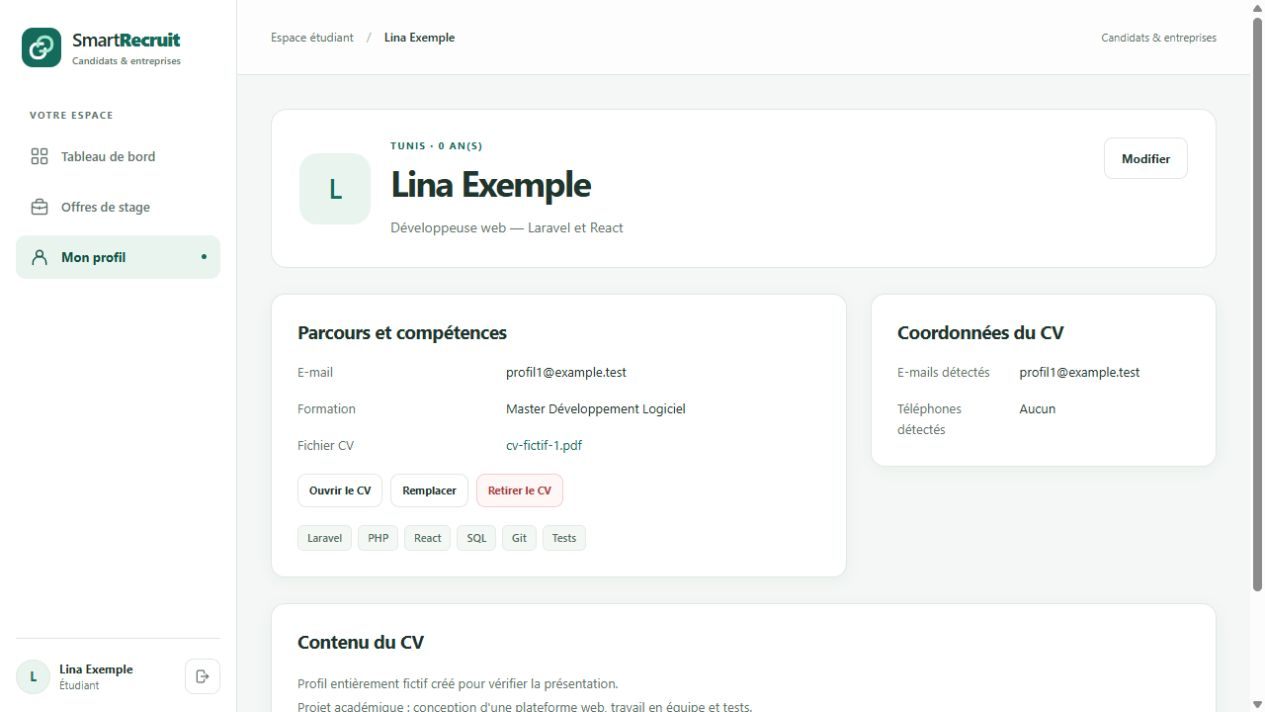
\includegraphics[width=.94\linewidth,height=.74\textwidth,keepaspectratio]{figures/screenshots/09-profil-etudiant.png}
\caption{Présentation du profil candidat et de ses compétences}
\label{fig:interface-09-profil-etudiant}\end{figure}
\end{landscape}

\begin{landscape}
\subsection{Catalogue des offres}
{\small\setstretch{1.05}
Les offres sont présentées avec les informations utiles à leur comparaison et un accès au détail. Des indicateurs de compatibilité et de suivi peuvent accompagner les résultats. Les valeurs visibles ici appartiennent au jeu illustratif ; elles ne mesurent pas la précision du moteur.\par}


\begin{figure}[H]\centering
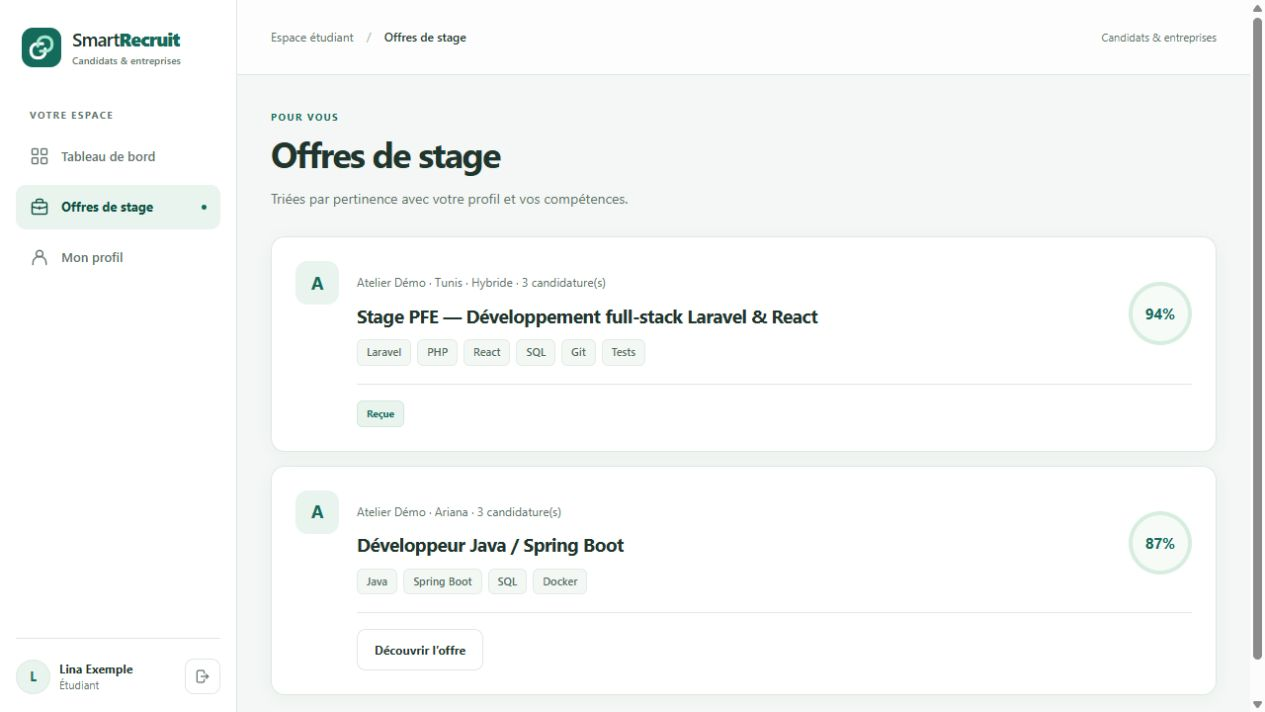
\includegraphics[width=.94\linewidth,height=.74\textwidth,keepaspectratio]{figures/screenshots/06-offres-etudiant.png}
\caption{Catalogue des offres dans l'espace candidat}
\label{fig:interface-06-offres-etudiant}\end{figure}
\end{landscape}

\begin{landscape}
\subsection{Détail d'une offre}
{\small\setstretch{1.05}
La page de détail expose la mission, les exigences et les informations de l'entreprise. Elle replace le rapprochement dans le contexte de l'offre et restitue la situation du candidat lorsqu'une candidature existe déjà. L'utilisateur peut ainsi comprendre le contenu du poste avant de poursuivre son suivi.\par}


\begin{figure}[H]\centering
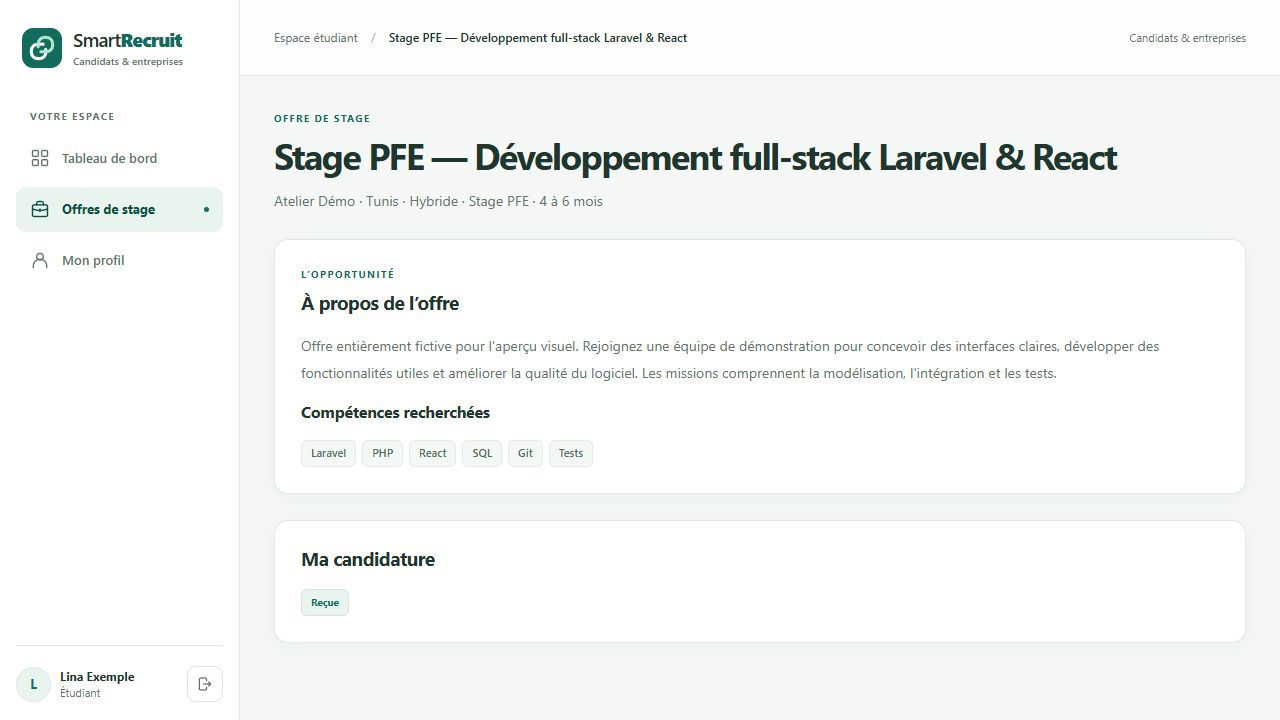
\includegraphics[width=.94\linewidth,height=.74\textwidth,keepaspectratio]{figures/screenshots/07-detail-offre.png}
\caption{Consultation d'une offre et de ses exigences}
\label{fig:interface-07-detail-offre}\end{figure}
\end{landscape}

\begin{landscape}
\subsection{Espace recruteur}
{\small\setstretch{1.05}
Le tableau de bord recruteur synthétise l'activité de ses offres et oriente vers leur gestion. Les filtres et les accès au vivier structurent le travail de consultation. Cette vue met en relation les cartes K05, K08 et K09, consacrées aux offres, aux décisions et au suivi.\par}


\begin{figure}[H]\centering
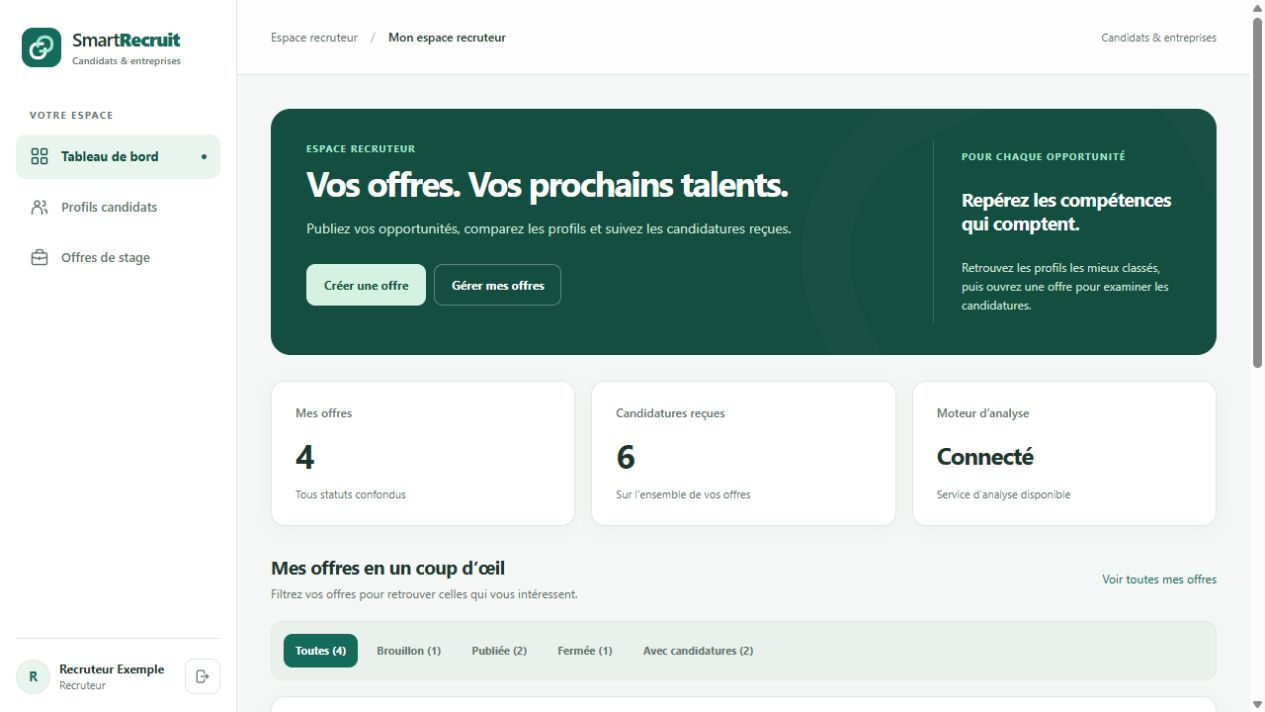
\includegraphics[width=.94\linewidth,height=.74\textwidth,keepaspectratio]{figures/screenshots/04-espace-recruteur.png}
\caption{Tableau de bord du recruteur}
\label{fig:interface-04-espace-recruteur}\end{figure}
\end{landscape}

\begin{landscape}
\subsection{Création d'une offre}
{\small\setstretch{1.05}
Le formulaire permet de décrire une opportunité et les compétences recherchées. La capture montre sa partie supérieure, avec les premiers champs nécessaires à la publication. Les informations saisies alimentent ensuite la consultation de l'offre et sa comparaison avec les profils.\par}


\begin{figure}[H]\centering
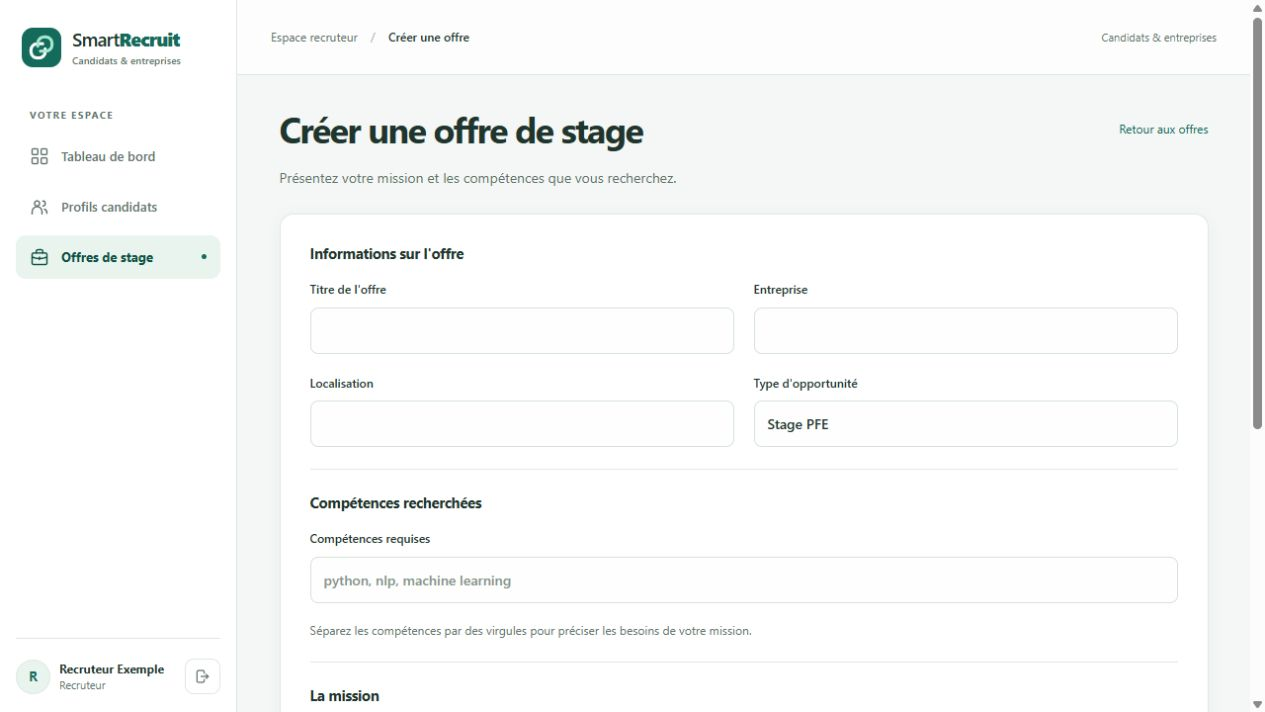
\includegraphics[width=.94\linewidth,height=.74\textwidth,keepaspectratio]{figures/screenshots/10-creation-offre.png}
\caption{Partie supérieure du formulaire de création d'une offre}
\label{fig:interface-10-creation-offre}\end{figure}
\end{landscape}

\begin{landscape}
\subsection{Vivier des candidats}
{\small\setstretch{1.05}
La liste des profils permet au recruteur de parcourir le vivier et d'accéder aux fiches détaillées. Les informations synthétiques facilitent une première lecture des parcours. La présence d'une personne dans ce vivier ne signifie pas qu'elle a postulé à une offre donnée.\par}


\begin{figure}[H]\centering
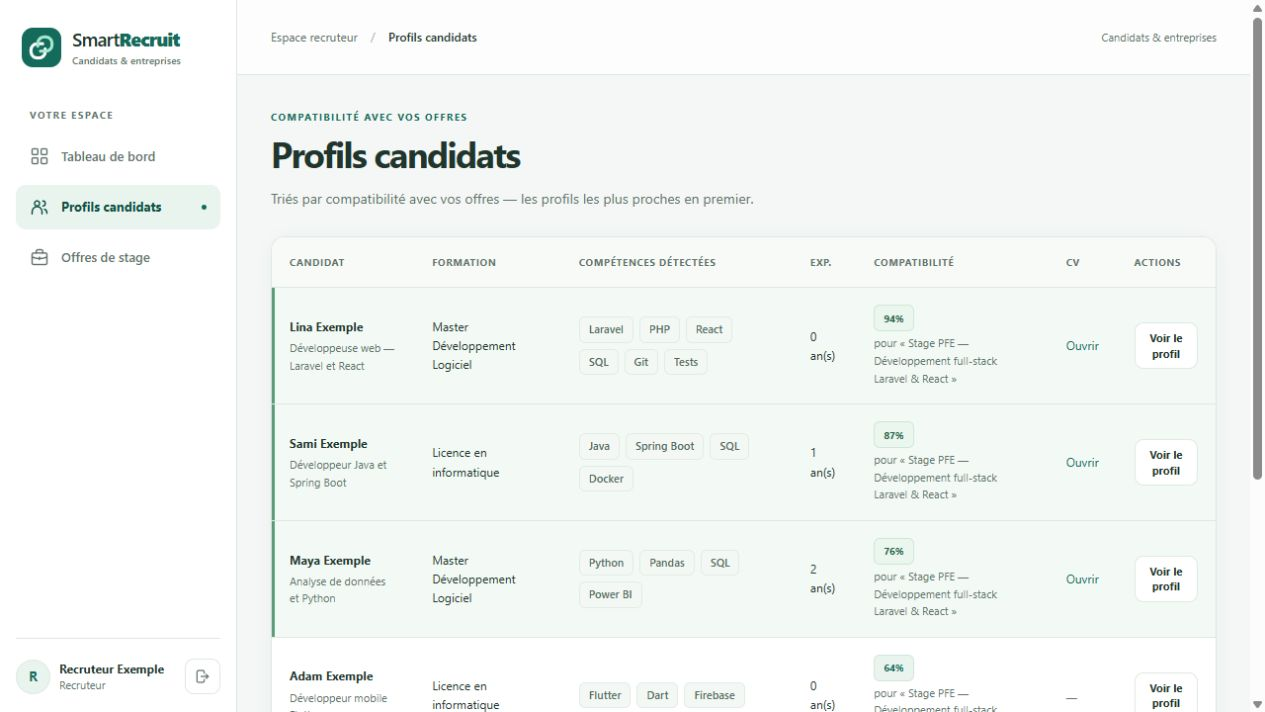
\includegraphics[width=.94\linewidth,height=.74\textwidth,keepaspectratio]{figures/screenshots/12-profils.png}
\caption{Consultation du vivier de profils par le recruteur}
\label{fig:interface-12-profils}\end{figure}
\end{landscape}

\begin{landscape}
\subsection{Classement pour une offre}
{\small\setstretch{1.05}
Le classement associe chaque profil à un score et à des éléments d'explication, notamment les compétences rapprochées ou manquantes. Les actions de décision concernent les candidatures existantes. La capture est centrée sur cette section de la page ; les scores sont des valeurs de démonstration.\par}


\begin{figure}[H]\centering
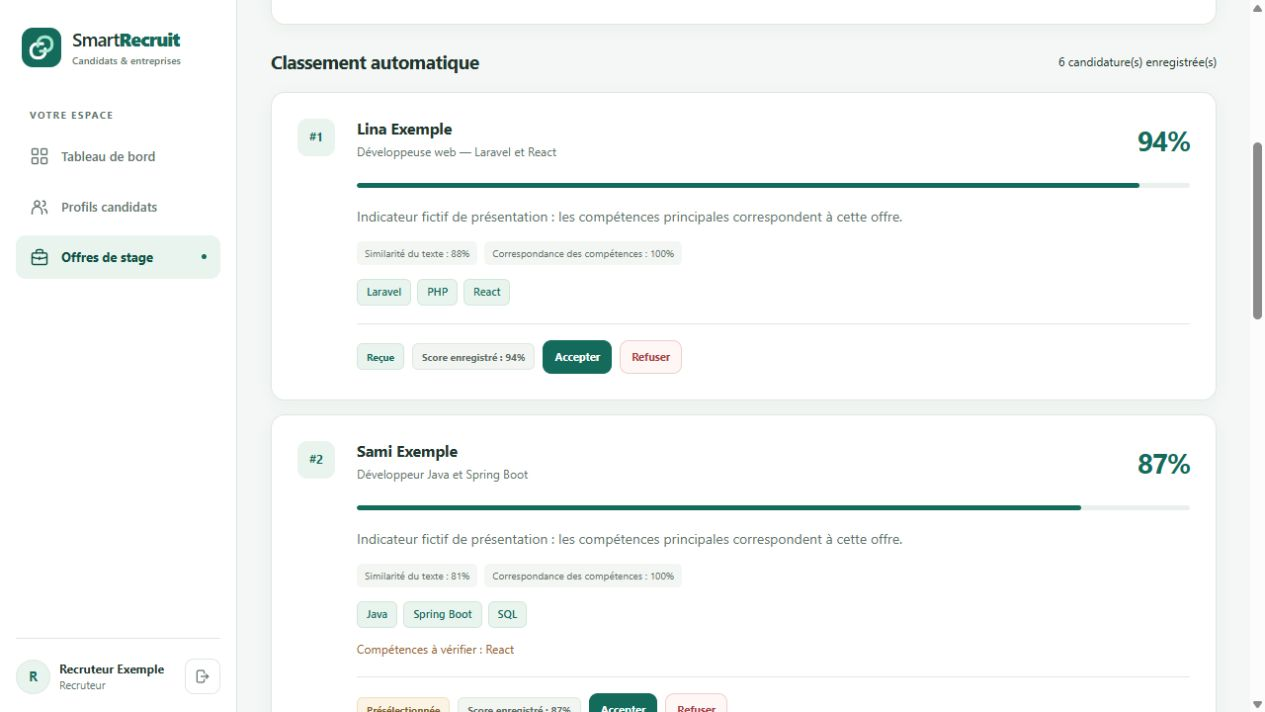
\includegraphics[width=.94\linewidth,height=.74\textwidth,keepaspectratio]{figures/screenshots/08-classement.png}
\caption{Section de classement des profils pour une offre}
\label{fig:interface-08-classement}\end{figure}
\end{landscape}

\begin{landscape}
\subsection{Supervision administrative}
{\small\setstretch{1.05}
L'espace administrateur fournit une vue transversale des comptes, des offres et des candidatures. Ses accès regroupent les fonctions de supervision et de gestion qui dépassent le périmètre d'un recruteur. Cette séparation rend visibles les responsabilités propres au troisième acteur UML.\par}


\begin{figure}[H]\centering
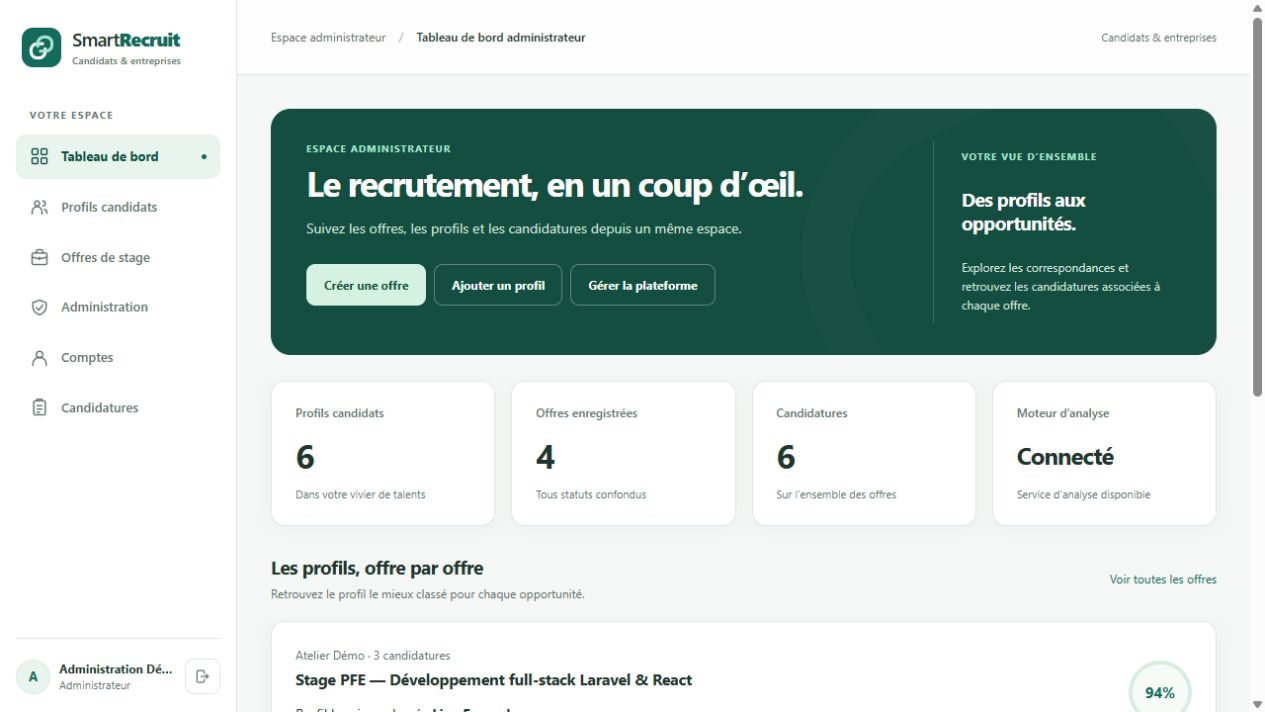
\includegraphics[width=.94\linewidth,height=.74\textwidth,keepaspectratio]{figures/screenshots/03-espace-administrateur.png}
\caption{Tableau de bord de l'administrateur}
\label{fig:interface-03-espace-administrateur}\end{figure}
\end{landscape}

\begin{landscape}
\subsection{Gestion des candidatures}
{\small\setstretch{1.05}
La liste administrative rassemble les candidatures, leur statut et les opérations de gestion. Les filtres permettent de retrouver les éléments actifs ou supprimés logiquement. Le statut métier et la présence dans la corbeille sont deux informations distinctes, conformément au diagramme d'états.\par}


\begin{figure}[H]\centering
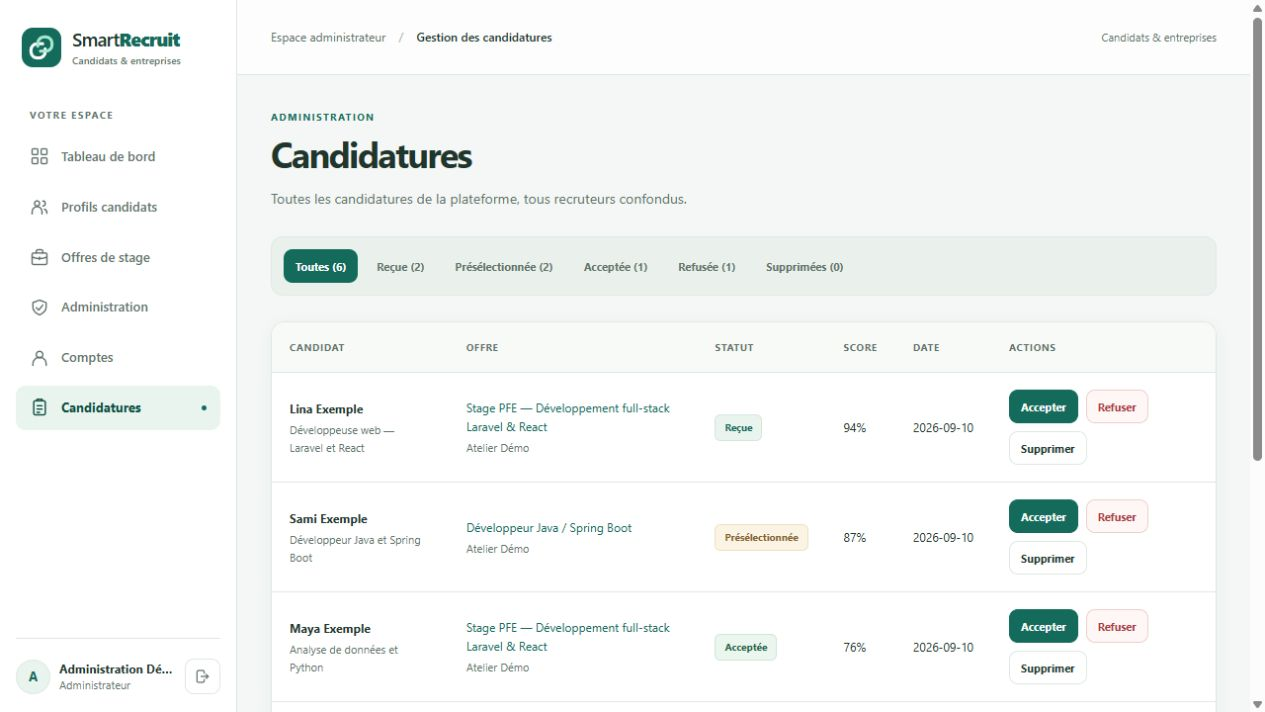
\includegraphics[width=.94\linewidth,height=.74\textwidth,keepaspectratio]{figures/screenshots/11-candidatures.png}
\caption{Suivi et gestion administrative des candidatures}
\label{fig:interface-11-candidatures}\end{figure}
\end{landscape}

